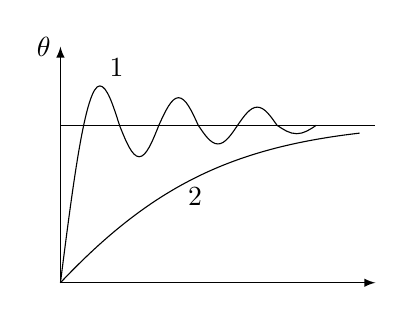
\begin{tikzpicture}

\coordinate (O) at (0, 0);

\begin{scope}[-latex]
\draw (O)--(4, 0);
\draw (O)--(0, 3)node[left]{$\theta$};
\end{scope}

\draw (0, 2)--+(4, 0);
\draw (O) to[bend left=20] node[below]{\maru{2}} (3.8, 1.9);

\draw (O) sin (0.5, 2.5)node[above right]{\maru{1}} cos (0.75, 2) sin (1, 1.6) cos (1.25, 2);
\foreach \x in {1.25, 2.25}{%
	\draw (\x, 2) sin (\x + 1/4, 2.5-0.12*\x) cos (\x + 1/2, 2) sin (\x + 3/4, 1.6+0.13*\x) cos (\x + 1, 2);
	}

\end{tikzpicture}
